\section{So sánh ViT và CNN: Khi nào nên dùng cái nào?}
\label{sec:vit_vs_cnn_comparison}

\subsection{Giới thiệu}
\label{subsec:comparison_intro}

Sau hơn một thập kỷ kể từ bước đột phá của AlexNet, \textbf{Mạng Nơ-ron Tích chập (CNN)} đã trở thành nền tảng chủ đạo của thị giác máy tính. Tuy nhiên, sự xuất hiện của \textbf{Vision Transformer (ViT)} vào năm 2020 đã đặt ra một cách tiếp cận hoàn toàn khác: thay vì xây dựng biểu diễn từ các tương tác cục bộ, ViT sử dụng cơ chế \textbf{self-attention toàn cục} để mô hình hóa trực tiếp quan hệ giữa mọi vùng ảnh.

Hai kiến trúc này không chỉ khác nhau về mặt kỹ thuật, mà còn phản ánh hai triết lý học biểu diễn:
\begin{itemize}
	\item CNN: học từ \textbf{cấu trúc không gian có sẵn} (strong inductive bias)
	\item ViT: học từ \textbf{dữ liệu} (data-driven representation learning)
\end{itemize}

Sự khác biệt này dẫn đến những hành vi rất khác nhau khi thay đổi quy mô dữ liệu, tài nguyên tính toán và mục tiêu ứng dụng. Phần này sẽ phân tích sâu các yếu tố đó, từ đó đưa ra một cách nhìn hệ thống để lựa chọn kiến trúc phù hợp.

---

\subsection{Một góc nhìn thống nhất}
\label{subsec:unified_view}

Có thể diễn giải CNN và ViT dưới một framework chung:

\begin{center}
	\textit{Biểu diễn thị giác = Feature Extraction + Token Mixing + Channel Mixing}
\end{center}

Trong đó:
\begin{itemize}
	\item \textbf{Feature Extraction:} chuyển ảnh thành các đặc trưng ban đầu
	\item \textbf{Token Mixing:} trao đổi thông tin giữa các vị trí không gian
	\item \textbf{Channel Mixing:} biến đổi theo chiều đặc trưng (MLP/FFN)
\end{itemize}

Sự khác biệt cốt lõi nằm ở \textbf{token mixing}:
\begin{itemize}
	\item CNN: mixing cục bộ (convolution)
	\item ViT: mixing toàn cục (self-attention)
\end{itemize}

Từ góc nhìn này, CNN và ViT không phải là hai họ hoàn toàn khác biệt, mà là hai cách cài đặt khác nhau của cùng một bài toán.

---

\subsection{Đánh giá Mạng Nơ-ron Tích chập (CNN)}
\label{subsec:cnn_evaluation}

\subsubsection{Ưu điểm}

\begin{description}
	\item[Thiên kiến quy nạp mạnh:]  
	CNN giả định rằng cấu trúc không gian là quan trọng. Hai giả định chính là:
	\begin{itemize}
		\item \textbf{Locality:} các pixel gần nhau có quan hệ mạnh hơn
		\item \textbf{Translation equivariance:} đặc trưng không phụ thuộc vị trí tuyệt đối
	\end{itemize}
	Điều này giúp mô hình học nhanh và ổn định ngay cả khi dữ liệu hạn chế.
	
	\item[Hiệu quả tính toán:]  
	Convolution có độ phức tạp tuyến tính theo số pixel và được tối ưu mạnh trên phần cứng.  
	Điều này giúp CNN phù hợp với các hệ thống yêu cầu độ trễ thấp.
	
	\item[Biểu diễn phân cấp tự nhiên:]  
	CNN xây dựng đặc trưng từ thấp đến cao (edge $\rightarrow$ texture $\rightarrow$ object), rất phù hợp cho các bài toán dense prediction.
\end{description}

\subsubsection{Hạn chế}

\begin{description}
	\item[Khó mô hình hóa quan hệ tầm xa:]  
	Thông tin phải đi qua nhiều lớp mới kết nối được các vùng xa nhau, dẫn đến suy giảm hiệu quả.
	
	\item[Thiếu thích ứng theo nội dung:]  
	Kernel là tĩnh sau khi huấn luyện, không thay đổi theo từng ảnh đầu vào.
\end{description}

\begin{mdframed}[style=infobox]
	CNN phù hợp khi dữ liệu hạn chế, yêu cầu tính toán thấp, hoặc cần suy luận thời gian thực.
\end{mdframed}

---

\subsection{Đánh giá Vision Transformer (ViT)}
\label{subsec:vit_evaluation}

\subsubsection{Ưu điểm}

\begin{description}
	\item[Khả năng mô hình hóa toàn cục:]  
	Self-attention cho phép mọi patch tương tác trực tiếp, giúp nắm bắt cấu trúc ngữ nghĩa phức tạp.
	
	\item[Khả năng mở rộng theo dữ liệu:]  
	Hiệu năng của ViT tăng mạnh khi quy mô dữ liệu và mô hình tăng, phù hợp với các hệ thống lớn.
	
	\item[Kiến trúc thống nhất:]  
	Transformer cung cấp một framework chung cho đa phương thức (vision, language, audio), tạo điều kiện cho các mô hình nền tảng.
\end{description}

\subsubsection{Hạn chế}

\begin{description}
	\item[Phụ thuộc dữ liệu lớn:]  
	Không có inductive bias khiến ViT cần nhiều dữ liệu để học các quy luật cơ bản.
	
	\item[Chi phí tính toán cao:]  
	Self-attention có độ phức tạp bậc hai theo số patch, gây khó khăn với ảnh độ phân giải cao.
\end{description}

\begin{mdframed}[style=infobox]
	ViT phù hợp khi có dữ liệu lớn, tài nguyên mạnh, và mục tiêu là đạt hiệu năng tối đa.
\end{mdframed}

---

\subsection{Phân tích theo quy mô dữ liệu và tài nguyên}
\label{subsec:scaling_analysis}

Một cách nhìn quan trọng là xem hành vi của hai mô hình theo quy mô:

\begin{itemize}
	\item \textbf{Dữ liệu nhỏ:}  
	CNN thường vượt trội nhờ inductive bias giúp học nhanh và tránh overfitting.
	
	\item \textbf{Dữ liệu lớn:}  
	ViT dần vượt lên do khả năng học biểu diễn linh hoạt hơn.
	
	\item \textbf{Tài nguyên hạn chế:}  
	CNN có lợi thế rõ rệt về tốc độ và chi phí.
	
	\item \textbf{Tài nguyên dồi dào:}  
	ViT khai thác tốt hơn scaling law của deep learning.
\end{itemize}

\begin{center}
	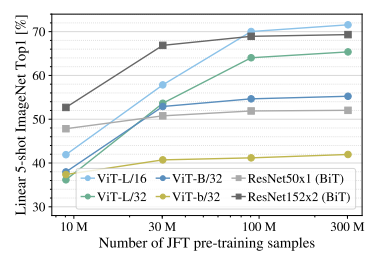
\includegraphics[width=0.9\textwidth]{images/cnn_vs_vit_performance_datasize.png}
	\captionof{figure}{So sánh hiệu năng theo quy mô dữ liệu}
\end{center}

---

\subsection{Mô hình Lai: Điểm cân bằng thực tiễn}
\label{subsec:hybrid_model_balance}

Các mô hình lai xuất hiện như một hệ quả tự nhiên của việc kết hợp hai cơ chế:

\begin{itemize}
	\item sử dụng CNN để xử lý ảnh ở độ phân giải cao
	\item sử dụng Transformer để xử lý biểu diễn ngữ nghĩa
\end{itemize}

Các kiến trúc như CoAtNet, MobileViT hay ConvNeXt cho thấy:
\begin{itemize}
	\item không cần lựa chọn tuyệt đối giữa CNN và ViT
	\item việc phân bổ đúng vai trò quan trọng hơn bản thân cơ chế
\end{itemize}

Trong thực tế, các mô hình lai thường đạt:
\begin{itemize}
	\item hiệu năng gần ViT
	\item chi phí gần CNN
\end{itemize}

---

\subsection{Hướng dẫn lựa chọn kiến trúc}
\label{subsec:practical_guidelines}

Từ các phân tích trên, có thể đưa ra một số nguyên tắc lựa chọn:

\begin{itemize}
	\item \textbf{Chọn CNN khi:}
	\begin{itemize}
		\item dữ liệu hạn chế
		\item yêu cầu thời gian thực
		\item triển khai trên thiết bị biên
	\end{itemize}
	
	\item \textbf{Chọn ViT khi:}
	\begin{itemize}
		\item có dữ liệu lớn hoặc pretraining mạnh
		\item cần hiệu năng tối đa
		\item làm việc với mô hình đa phương thức
	\end{itemize}
	
	\item \textbf{Chọn Hybrid khi:}
	\begin{itemize}
		\item cần cân bằng giữa hiệu năng và chi phí
		\item hệ thống thực tế có ràng buộc tài nguyên
	\end{itemize}
\end{itemize}

---

\subsection{Kết luận: Từ đối đầu đến hội tụ}
\label{subsec:unified_future_conclusion}

Sự phát triển của CNN và Transformer không dẫn đến việc một kiến trúc thay thế hoàn toàn kiến trúc còn lại, mà dẫn đến một sự hội tụ.

Thay vì xem chúng như hai hướng đối lập, có thể hiểu rằng:
\begin{itemize}
	\item CNN cung cấp cấu trúc hiệu quả để xử lý không gian
	\item Transformer cung cấp cơ chế linh hoạt để mô hình hóa quan hệ
\end{itemize}

Các kiến trúc hiện đại ngày càng kết hợp hai yếu tố này trong cùng một framework, nơi convolution, attention và các phép biến đổi khác chỉ còn là những lựa chọn thiết kế trong một không gian kiến trúc rộng hơn.

Điều này phản ánh một xu hướng chung trong học sâu:  
\begin{center}
	\textit{từ các mô hình chuyên biệt sang các hệ thống có thể cấu hình linh hoạt theo dữ liệu và phần cứng}
\end{center}

\section*{Tài liệu tham khảo}
\begin{itemize}
	\item[1] Dosovitskiy, A., Beyer, L., Kolesnikov, A., Weissenborn, D., Zhai, X., Unterthiner, T., ... \& Houlsby, N. (2020). An image is worth 16x16 words: Transformers for image recognition at scale. \textit{arXiv preprint arXiv:2010.11929}. (Paper gốc về ViT, đặt ra sự so sánh trực tiếp với các kiến trúc CNN).
	\item[2] He, K., Zhang, X., Ren, S., \& Sun, J. (2016). Deep residual learning for image recognition. In \textit{Proceedings of the IEEE conference on computer vision and pattern recognition (CVPR)}. (Đại diện tiêu biểu cho kiến trúc CNN hiện đại).
	\item[3] Liu, Z., Mao, H., Wu, C. Y., Feichtenhofer, C., Darrell, T., \& Xie, S. (2022). A convnet for the 2020s. In \textit{Proceedings of the IEEE/CVF conference on computer vision and pattern recognition (CVPR)}. (Paper về ConvNeXt, một ví dụ điển hình của việc kết hợp triết lý thiết kế từ cả hai trường phái).
	\item[4] Dai, Z., Liu, H., Le, Q. V., \& Tan, M. (2021). Coatnet: Marrying convolution and attention for all data sizes. In \textit{Advances in Neural Information Processing Systems (NeurIPS)}. (Một ví dụ về kiến trúc lai tuần tự hiệu quả).
	\item[5] Radford, A., Kim, J. W., Hallacy, C., Ramesh, A., Goh, G., Agarwal, S., ... \& Sutskever, I. (2021). Learning transferable visual models from natural language supervision. In \textit{International Conference on Machine Learning (ICML)}. (Ví dụ về sức mạnh của kiến trúc Transformer trong các tác vụ đa phương thức và học tổng quát).
\end{itemize}